\titledquestion{1-Median with Manhattan-Distance}

Mr. B. Rentzen is a fruit farmer and supplier for a nearby producer of a delicious fruit schnapps. The supply contract covers his entire annual harvest minus a portion that fluctuates annually and does not meet the quality standards applicable to schnapps production. So far, it has been sufficient for Mr. Rentzen to presort the harvest and to make it available for collection in the immediate vicinity of each of his eight fruit fields. He has identified the location of them by the coordinates $(a_i,b_i)=(1,1),(1,5),(2,3),(2,2),(4,3),(4,4),(5,5),$ $(5,1)$.\\ 
As of next year, the Schnapps Distillery requires that the pick-ups must be clustered at exactly \emph{one} location. Mr. B. Rentzen realizes that in the future he will have to provide additional transportation effort for the collection of the presorted goods. To keep this as low as possible, he is currently looking for the best location for the new collection point.\\
Mr. Rentzen estimates that he can sell two tons of marketable fruit per year from each field, i.e., $w_i=2$ [t/Y] for all $i=1,\ldots,8$. Given the road network in the area, the distance between a location $(a_i,b_i)$ and a potential collection point $(x,y)$ can be approximated as Manhattan distance (in km).

\begin{enumerate}
	\item Separate the objective function into its one-dimensional components and plot them for $1 \leq x\leq 5$ and $1\leq y\leq 5$. What are the coordinates of the optimal collection point location if you solve the problem in $\R^2$?
	\begin{solution}
	
	\uline{Input/Given:}\\
	 Finite set of  Mr. Rentzens eight fruit fields:\\
		\begin{itemize}
			\item Indices $i\in\left\{1,2,3,4,5,6,7,8\right\}$
			\item Coordinates $\left(1,1\right)$, $\left(1,5\right)$, $\left(2,3\right)$, $\left(2,2\right)$, $\left(4,3\right)$, $\left(4,4\right)$, $\left(5,5\right)$, $\left(5,1\right)$			
			\item Marketable amount of fruit $w_i=2$ $\left[t/Y\right]$ for all $i=1,\ldots,8$ (also called `weights')
			\item Number of sought collection points for the bundled total delivery quantity $p=1$
			\item Distance function: Manhattan distance
		\end{itemize}
	\uline{Output/Wanted:}\\
\phantom{	A location in $(x,y) \in \R^2$ such that the sum of the $w_i$ weighted distances between the collection locations and the collection point is minimal}
	
	\underline{Model:}

		$$\min_{(x,y)\in\R^2} F\left(x,y\right)=\min_{(x,y)\in\R^2} \sum_{i=1}^m w_i d^1\left(\left(x,y\right),\left(a_i,b_i\right)\right)$$
		
		Due to the form of the Manhattan distance function (sum in brackets), the objective function can be rearranged so that the following is valid:\\
		
	\[F\left(x,y\right)=\sum_{i=1}^m w_i \left(\left|x-a_i\right|+\left|y-b_i\right|\right)=\phantom{\sum_{i=1}^m w_i \left(\left|x-a_i\right|\right)+\sum_{i=1}^m w_i \left(\left|y-b_i\right|\right)=F_1\left(x\right)+F_2\left(y\right)}
\]
			
		Which values of $x\in \mathbb{R}$ must be considered? \\
		\phantom{$\{x|(x,y) \in C\} = \{1,2,3,4,5\}$} \\ \\
		Graphical representation of $F_1\left(x\right)$:\\
		\begin{center}
			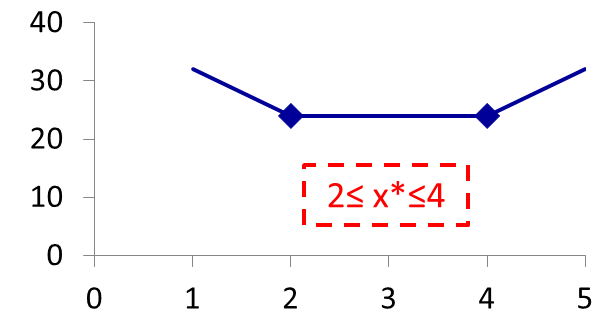
\includegraphics[scale=0.5]{Uebungen/figures/A_1_1_Fx}
		\end{center}
		Calculation of the possible $x$ values for the collection point:\\
		\begin{tabular}{ll}
		$x=1$&$F_1(1)=2\left|1-1\right|+2\left|1-1\right|+2\left|1-2\right|+2\left|1-2\right|+2\left|1-4\right|+2\left|1-4\right|+2\left|1-5\right|+2\left|1-5\right|=32$\\
		$x=2$&$F_1(2)=2\left|2-1\right|+2\left|2-1\right|+2\left|2-2\right|+2\left|2-2\right|+2\left|2-4\right|+2\left|2-4\right|+2\left|2-5\right|+2\left|2-5\right|=24$\\
		$x=3$&$F_1(3)=2\left|3-1\right|+2\left|3-1\right|+2\left|3-2\right|+2\left|3-2\right|+2\left|3-4\right|+2\left|3-4\right|+2\left|3-5\right|+2\left|3-5\right|=24$\\
		$x=4$&$F_1(4)=2\left|4-1\right|+2\left|4-1\right|+2\left|4-2\right|+2\left|4-2\right|+2\left|4-4\right|+2\left|4-4\right|+2\left|4-5\right|+2\left|4-5\right|=24$\\
		$x=5$&$F_1(5)=2\left|5-1\right|+2\left|5-1\right|+2\left|5-2\right|+2\left|5-2\right|+2\left|5-4\right|+2\left|5-4\right|+2\left|5-5\right|+2\left|5-5\right|=32$\\
		\end{tabular}
	\vspace{1cm}
		
		Graphical representation of $F_2\left(y\right)$:\\
		
		Which values of $y\in \mathbb{R}$ must be considered? \\
		\phantom{$\{y| (x,y) \in C\} = \{1,2,3,4,5\}$} \\ 
		\vspace{0.3cm}
		
		\begin{center}
			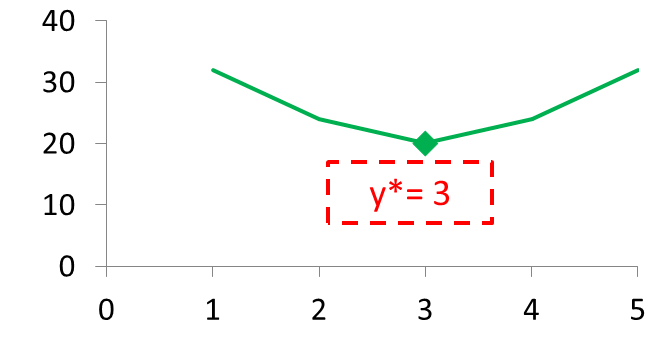
\includegraphics[scale=0.5]{Uebungen/figures/A_1_1_Fy}
		\end{center}
		Calculation of the possible $x$ values for the collection point:\\
		\begin{tabular}{ll}
		$y=1$&$F_2(1)=2\left|1-1\right|+2\left|1-5\right|+2\left|1-3\right|+2\left|1-2\right|+2\left|1-3\right|+2\left|1-4\right|+2\left|1-5\right|+2\left|1-1\right|=32$\\
		$y=2$&$F_2(2)=2\left|2-1\right|+2\left|2-5\right|+2\left|2-3\right|+2\left|2-2\right|+2\left|2-3\right|+2\left|2-4\right|+2\left|2-5\right|+2\left|2-1\right|=24$\\
		$y=3$&$F_2(3)=2\left|3-1\right|+2\left|3-5\right|+2\left|3-3\right|+2\left|3-2\right|+2\left|3-3\right|+2\left|3-4\right|+2\left|3-5\right|+2\left|3-1\right|=20$\\
		$y=4$&$F_2(4)=2\left|4-1\right|+2\left|4-5\right|+2\left|4-3\right|+2\left|4-2\right|+2\left|4-3\right|+2\left|4-4\right|+2\left|4-5\right|+2\left|4-1\right|=24$\\
		$y=5$&$F_2(5)=2\left|5-1\right|+2\left|5-5\right|+2\left|5-3\right|+2\left|5-2\right|+2\left|5-3\right|+2\left|5-4\right|+2\left|5-5\right|+2\left|5-1\right|=32$\\
		\end{tabular}
	\end{solution}
	\item Identify key characteristics of the functions shown, especially with regard to the location of the optimal sites!
	\begin{solution}
	\uline{Properties of $F_1\left(x\right)$ and $F_2\left(y\right)$}
		\begin{itemize}
			\item The functions are piece-wise linear, i.e.	
				\begin{itemize}
					\item \phantom{ the functions increase or decrease linearly between customer locations $a_i$ and $b_i$ in $x$ and $y$, respectively.}
					\item \phantom{ the functions are continuous, but not (everywhere) differentiable (specifically, not at the (customer) locations).}
					\item \phantom{ minima lie between sub-intervals with alternating slope signs.}
				\end{itemize}
			\item  The functions are convex, i.e. local Minima are also global Minima.
		\end{itemize}
	\end{solution}
	\item Determine the optimal location arithmetically. Furthermore, compute the additional transport effort Mr. Rentzen must provide in [tkm/Y] for the chosen optimal location. 
	\begin{solution}
	\uline{Procedure to determine a 1-median in $\mathbb{R}$:}\\
		\begin{enumerate}
			\item Calculate half of the total delivery quantity $\frac{W}{2}=\frac{\sum_{i=1}^m w_i}{2}$.
			\item Sort the possible locations in ascending order of $a_i$ and $b_i$ separately.
			\item Use the sorted list to calculate the accumulated quantities (`weights') $\sum_{k=1}^i w_k$.\\
			\item Use the list to search for coordinates $a_i$ and $b_i$ that have the smallest accumulated quantity, which is also greater or equal to $\frac{W}{2}$.
		\end{enumerate}
	\uline{Note:} If equality is satisfied for a customer $i^*$, then all points between customer locations $i^*$ and $i^*+1$ are optimal, i.e. $x^* \in \left[a_{i^*},a_{i^*+1}\right]$.\\
	
	Calculate: $\frac{W}{2}= \frac{2\cdot8}{2}=8$.\\
	
	\begin{tabular}{cccc|cccc}
	$i$&$a_i$&$w_i$&$\sum_k^i w_k$ &$i$&$b_i$&$w_i$&$\sum_k^i w_k$\\
	\hline
	\phantom{1}&\phantom{1}&\phantom{2}&\phantom{2} &1&\phantom{1}&\phantom{2}&\phantom{2}\\
	\phantom{2}&\phantom{1}&\phantom{2}&\phantom{4} &\phantom{8}&\phantom{1}&\phantom{2}&\phantom{4}\\
	\phantom{3}&\phantom{2}&\phantom{2}&\phantom{6} &\phantom{4}&\phantom{2}&\phantom{2}&\phantom{6}\\
	\phantom{4}&\phantom{\red{2}}&\phantom{2}&\phantom{\red{8=W/2}} &\phantom{3}&\phantom{\red{3}}&\phantom{2}&\phantom{\red{8=W/2}}\\
	\phantom{5}&\phantom{\red{4}}&\phantom{2}&\phantom{10} &\phantom{5}&\phantom{\red{3}}&\phantom{2}&\phantom{10}\\
	\phantom{6}&\phantom{4}&\phantom{2}&\phantom{12} &\phantom{6}&\phantom{4}&\phantom{2}&\phantom{12}\\
	\phantom{7}&\phantom{5}&\phantom{2}&\phantom{14} &\phantom{2}&\phantom{5}&\phantom{2}&\phantom{14}\\
	\phantom{8}&\phantom{5}&\phantom{2}&\phantom{16} &\phantom{7}&\phantom{5}&\phantom{2}&\phantom{16}\\
	\end{tabular}\\
	The coordinates of the optimal collection point are  \phantom{$x^*\in \left[2,4\right]$ and $y^*=3$}.\\
	
	Calculation of the transport performance for the chosen optimal location $(x^*,y^*)$:\\
	$F\left(x,y\right)=F\left(\phantom{2,3}\right)=\sum_{i=1}^8 w_i d^1\left(\left(\phantom{2,3}\right),\left(a_i,b_i\right)\right)=\sum_{i=1}^8 w_i \left(\left|\phantom{2}-a_i\right|+\left|\phantom{3}-b_i\right|\right)=\phantom{44}$\\
	\end{solution}
\end{enumerate}